\section{NET\_09 - BGP Security}

\subsection{Introduzione e contesto}

\subsubsection{Perché BGP security è ancora un problema rilevante}
Il \emph{Border Gateway Protocol} (BGP) è il protocollo cardine per l’instradamento \emph{inter-dominio}: consente agli \emph{Autonomous System} (AS) di scambiarsi informazioni di raggiungibilità e di applicare \emph{policy} di routing su scala Internet. Proprio perché governa la connettività globale, un singolo annuncio errato o malevolo può propagarsi rapidamente e generare impatti ampi: deviazione del traffico, perdita di connettività verso prefissi legittimi, detour e degradazione delle prestazioni.

La fragilità strutturale deriva dal modello originario di fiducia tra operatori: BGP non integra, di default, meccanismi forti per verificare l’autorità di un AS a originare un prefisso, né per garantire l’integrità del cammino dichiarato tramite \texttt{AS\_PATH}. Di conseguenza, la robustezza del routing dipende in larga parte da configurazioni coerenti, accordi tra reti e buone pratiche operative (filtri, policy di import/export e monitoraggio). Misconfigurazioni e comportamenti malevoli sfruttano lo stesso punto debole: annunci non corretti possono essere accettati e propagati come se fossero legittimi.

Un ulteriore elemento è che BGP si appoggia a una sessione affidabile su TCP (porta 179): l’interruzione della sessione o l’instabilità del control plane può causare ritiri massivi di rotte e riconvergenze, con effetti percepibili in termini di disponibilità.

\begin{figure}[H]
\centering
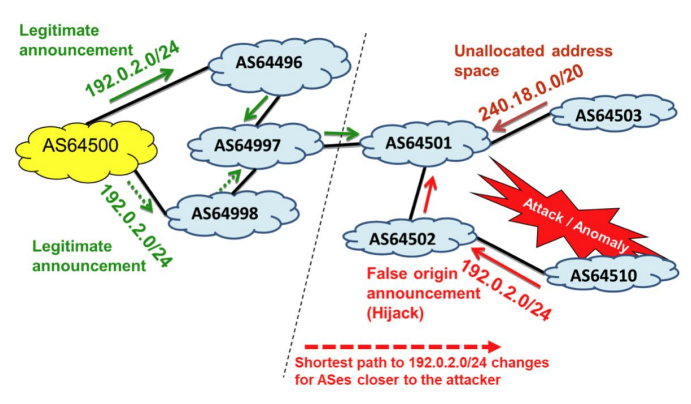
\includegraphics[width=0.80\textwidth]{immagini/NET_09/fig_bgphijack_example.png}
\caption{Esempio di \emph{prefix hijacking}: un AS non autorizzato origina un prefisso legittimo e può indurre una parte di Internet a selezionare un cammino verso il falso origin, causando \emph{misrouting} o \emph{blackholing}.}
\label{fig:bgp-prefix-hijack-example}
\end{figure}

\subsubsection{Panoramica delle minacce: control plane vs data plane}
Per organizzare l’analisi, è utile distinguere tra minacce al \emph{control plane} (informazioni di routing e stabilità) e minacce al \emph{data plane} (trasporto effettivo dei pacchetti). In questo quadro, il \emph{control channel} (la sessione BGP su TCP) è una componente critica: se la sessione cade, l’effetto operativo è immediato perché i peer ritirano le rotte apprese e la rete deve riconvergere.

Le minacce al \emph{control plane} includono fenomeni come \emph{prefix hijacking} (e la variante più impattante \emph{sub-prefix hijacking}), \emph{route leaks} (propagazioni oltre lo scope previsto dalle relazioni di peering/transit) e manipolazioni di attributi che influenzano la selezione del best path. Anche l’instabilità del routing (ad esempio \emph{route flapping}) può degradare la convergenza e aumentare il carico di controllo.

Le minacce al \emph{data plane} riguardano invece il traffico: attacchi volumetrici (DDoS), reflection/amplification e, più in generale, abusi che sfruttano la connettività. Nella pratica i due piani si combinano spesso: un hijack può facilitare deviazione o intercettazione del traffico, mentre un DDoS può essere amplificato o reso più difficile da mitigare da scelte di routing e peering.

\subsubsection{Riferimenti e best practice (idea generale)}
Nel materiale, le difese vengono presentate come un insieme di misure complementari. Una prima linea è l’hardening della sessione (protezione del canale TCP) per ridurre spoofing e interruzioni del peering. Una seconda linea è l’igiene operativa del routing: filtri e policy di import/export coerenti con il tipo di relazione (customer, provider, peer) per limitare errori e leak. Infine, una misura strutturale è la validazione dell’origine con RPKI e BGP Origin Validation, che rafforza la verifica di chi è autorizzato a originare un prefisso. In sintesi, l’approccio moderno è stratificato: controlli leggeri e operativi, più validazioni robuste quando disponibili, affiancati da monitoraggio e risposta agli incidenti.

\subsection{Vulnerabilità legate a IP/TCP e protezione della sessione BGP}

\subsubsection{Peer spoofing e attacchi di reset (TCP RST) / session disruption}
Poiché BGP opera sopra TCP (porta 179), la sicurezza della sessione tra peer è un requisito operativo fondamentale. Un avversario che conosca gli endpoint della sessione può tentare di \emph{spoofare} segmenti TCP facendoli apparire provenienti dal peer legittimo. Un caso tipico è l’iniezione di segmenti \texttt{RST}: se accettati, la sessione BGP viene abbattuta.

L’effetto è immediato: le rotte apprese vengono ritirate (\emph{withdraw}) e la connettività può degradare fino alla riconvergenza. Non è un attacco che “inventa” nuove rotte come un hijack, ma impatta direttamente la disponibilità e la stabilità del control plane, ed è per questo che vengono adottate contromisure dedicate sul canale di controllo.

\begin{figure}[H]
\centering
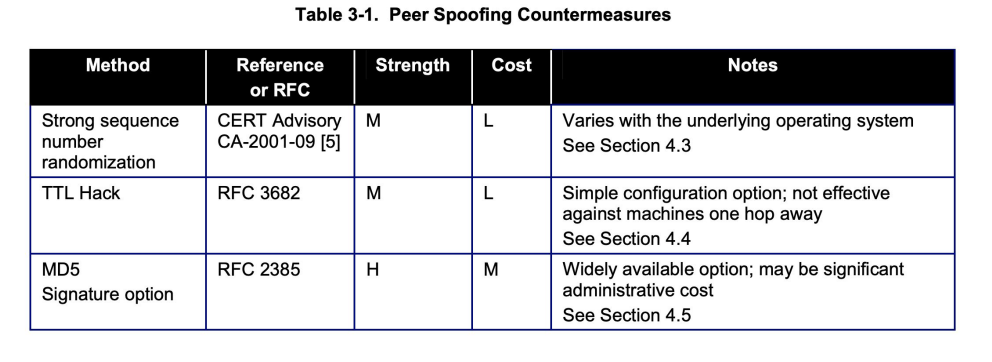
\includegraphics[width=0.75\textwidth]{immagini/NET_09/tab_peer_spoofing_countermeasures.png}
\caption{Sintesi delle principali contromisure contro \emph{peer spoofing} e \emph{TCP reset injection}: randomizzazione robusta dei sequence number, GTSM/TTL hack e autenticazione TCP (MD5 legacy).}
\label{fig:peer-spoofing-countermeasures}
\end{figure}

\subsubsection{Autenticazione a livello trasporto: TCP MD5 (legacy) e TCP-AO}
Una contromisura diretta consiste nell’autenticare i segmenti TCP della sessione BGP tramite un MAC calcolato con una chiave simmetrica condivisa tra peer. L’obiettivo è impedire a un avversario di iniettare segmenti validi senza conoscere la chiave, inclusi \texttt{RST} e \texttt{ACK} malevoli. La \emph{TCP MD5 option} è stata storicamente molto usata per BGP: è efficace come autenticazione, ma oggi è considerata una soluzione legacy, soprattutto per limiti operativi nella gestione e rotazione delle chiavi.

\emph{TCP-AO} rappresenta l’evoluzione moderna: supporta algoritmi più robusti e include meccanismi più adatti alla gestione del \emph{key rollover} su connessioni long-lived. Il limite resta principalmente operativo: la chiave deve essere gestita e configurata in modo coerente tra operatori. In ogni caso, TCP-MD5/TCP-AO forniscono autenticazione del canale (non necessariamente cifratura) e riducono in modo significativo la superficie di spoofing/reset.

\subsubsection{Generalized TTL Security Mechanism (GTSM / ``TTL hack'')}
Il \emph{TTL hack} (GTSM) sfrutta la semantica del campo TTL: ogni hop lo decrementa, quindi pacchetti provenienti da lontano arrivano con TTL più basso. In eBGP i peer sono tipicamente adiacenti: si imposta il TTL in uscita a 255 e si accettano solo pacchetti che arrivano con TTL coerente con una distanza massima attesa (ad esempio 255 per adiacenti, 254 se si ammette un hop intermedio). In questo modo, un attaccante remoto difficilmente può far arrivare pacchetti con TTL sufficientemente alto, anche conoscendo IP e porta del peer.

\subsubsection{Route flapping e Route Flap Damping (RFD)}
Una vulnerabilità importante, anche non intenzionale, è il \emph{route flapping}: una rotta viene ritirata e poi riannunciata ripetutamente. Ogni flap produce aggiornamenti e ritiri che possono propagarsi e costringere i router a ricalcoli frequenti. Se l’instabilità è elevata, il carico sul control plane aumenta e la convergenza peggiora, fino a instabilità percepibili dagli utenti (perdita di pacchetti, rallentamenti, interruzioni).

Il \emph{Route Flap Damping} (RFD) tenta di contenere il problema assegnando penalità agli eventi di flap, con decadimento nel tempo e soglie che portano alla soppressione temporanea di rotte instabili. Operativamente, va configurato con cautela: parametri troppo aggressivi possono causare soppressioni indesiderate e peggiorare la reachability, e in alcuni scenari l’instabilità può essere indotta per ottenere un effetto di DoS indiretto.

\subsubsection{IPsec per BGP: razionale e limiti pratici}
Proteggere la sessione BGP con IPsec è concettualmente possibile (autenticazione e, se desiderato, cifratura a livello rete), ma nella pratica è poco adottato sul peering inter-dominio. Le motivazioni principali sono operative: gestione e manutenzione delle Security Association, rekeying su sessioni long-lived, complessità di negoziazione e impatto di scalabilità in scenari con molti peer. Per questo, si preferiscono contromisure più leggere e ampiamente supportate (TCP-AO/MD5 legacy e GTSM), concentrando gli sforzi soprattutto sulle minacce del control plane (hijacking/leaks).

\subsection{Minacce al BGP control plane: hijacking e misrouting}

\subsubsection{Prefix hijacking e sub-prefix hijacking}
Si parla di \emph{prefix hijacking} quando un AS origina (per errore o in modo malevolo) un prefisso per cui non è autorizzato. In assenza di un controllo nativo e universalmente applicato sull’origine, l’annuncio può essere accettato e propagato, entrando nelle tabelle di routing di altri AS. A parità di prefisso, la selezione del best path dipende dalle policy locali e spesso anche da elementi come la “vicinanza” topologica o la lunghezza dell’\texttt{AS\_PATH}, quindi una parte di Internet può installare la rotta verso l’AS sbagliato, causando \emph{misrouting}.

La variante più impattante è il \emph{sub-prefix hijacking}: l’attaccante annuncia un prefisso più specifico contenuto in quello legittimo. Il motivo è nel forwarding IP: la regola del \emph{longest prefix match} privilegia la rotta più specifica, per cui un /28 può catturare traffico anche se il legittimo owner continua ad annunciare un /24.

\subsubsection{Conseguenze operative e casi reali}
Gli effetti vanno dal blackholing (DoS) a detour e degradazione prestazionale. In scenari più insidiosi, il traffico può transitare nella rete dell’attaccante, abilitando osservazione o intercettazione con reinoltro per ridurre la detection. Il materiale include anche esempi e incidenti reali che mostrano come hijack e leak non siano eventi rari e possano coinvolgere servizi ad alto traffico.

\subsection{Difese operative: Prefix (Route) Filtering}

\subsubsection{Principi: inbound/outbound filtering e approcci ``strict'' vs ``loose''}
Il \emph{prefix filtering} è una difesa operativa di base: in una relazione di peering esiste un insieme di annunci attesi, coerenti con quella relazione, e annunci non attesi che vanno rigettati. Per ridurre sia il rischio di essere colpiti sia quello di diventare sorgente di incidenti, i filtri vanno applicati in modo bidirezionale: in ingresso (inbound) per proteggere la propria rete da annunci anomali, e in uscita (outbound) per evitare di propagare errori o leak.

Si distinguono due impostazioni: lo \emph{strict filtering} (accetto solo ciò che è previsto per quel peer, tipicamente con allow-list per-peer) e il \emph{loose filtering} (quando non è possibile mantenere liste precise, si applicano filtri di igiene per eliminare categorie sicuramente anomale). Dal punto di vista operativo, lo strict è più robusto ma richiede manutenzione, mentre il loose resta utile per ridurre incidenti e abusi.

\subsubsection{Classi di filtri e punti chiave}
Il materiale raggruppa filtri tipici in classi: rigetto di prefissi non allocati o special-purpose, rigetto (o trattamento conservativo) di annunci dei propri prefissi ricevuti dall’esterno, limiti di specificità per ridurre la superficie del sub-prefix hijack, gestione prudente della default route e considerazioni specifiche per IXP LAN prefixes.

Il \emph{specificity limit} è una regola semplice ma efficace: in IPv4 è comune filtrare prefissi più specifici di /24 e in IPv6 più specifici di /48, salvo eccezioni concordate (ad esempio Flowspec in contesti di mitigazione DDoS). La default route, invece, è tipicamente filtrata in eBGP perché un annuncio improprio può attrarre grandi volumi di traffico; può essere accettata solo se prevista dall’accordo (es.\ customer stub che richiede solo default).

Negli IXP, dove si opera su una LAN di livello 2 condivisa, la reachability dell’IXP LAN prefix è utile anche per aspetti pratici come PMTUD in presenza di uRPF: per questo si accetta il LAN prefix annunciato dall’IXP e si evita che circolino più-specifici anomali di quel prefisso.

\subsection{RPKI e BGP Origin Validation (BGP-OV)}

\subsubsection{Perché serve RPKI e cosa contiene una ROA}
Storicamente, gli operatori hanno usato anche IRR per costruire filtri, ma la qualità dei dati può variare. RPKI introduce una base crittografica: tramite una \emph{ROA} si pubblica un binding tra prefisso e \emph{origin AS} autorizzato. Un elemento importante è il \texttt{maxlength}: specifica fino a che lunghezza sono ammessi i più-specifici del prefisso, distinguendo de-aggregazioni legittime da annunci sospetti.

\begin{figure}[H]
\centering
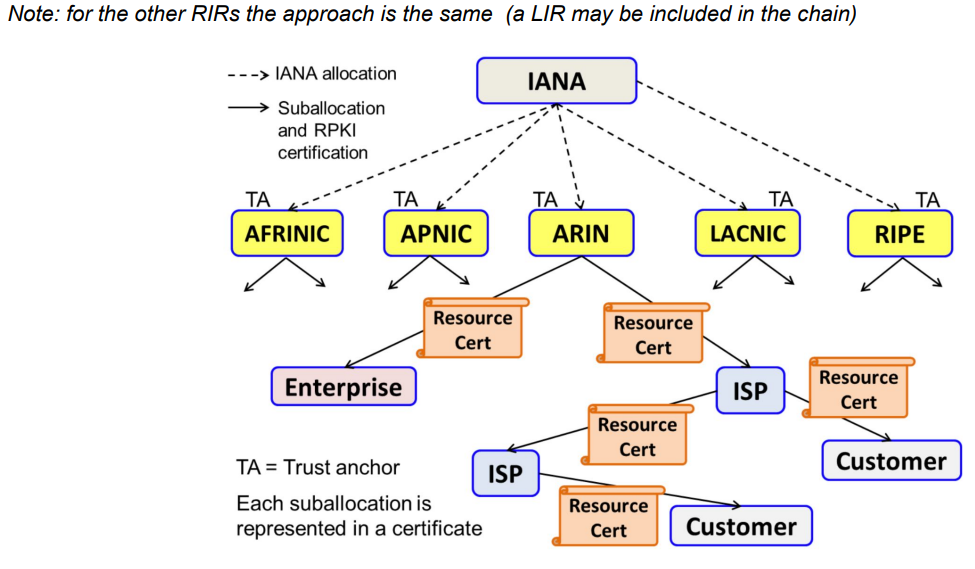
\includegraphics[width=0.85\textwidth]{immagini/NET_09/fig_rpki_chain_allocation.png}
\caption{Allocazione delle risorse e catena di certificazione in RPKI: IANA $\rightarrow$ RIR (trust anchor regionali) $\rightarrow$ ISP/enterprise $\rightarrow$ customer, con certificati che vincolano insiemi di prefissi e ASN.}
\label{fig:rpki-allocation-chain}
\end{figure}

\begin{figure}[H]
\centering
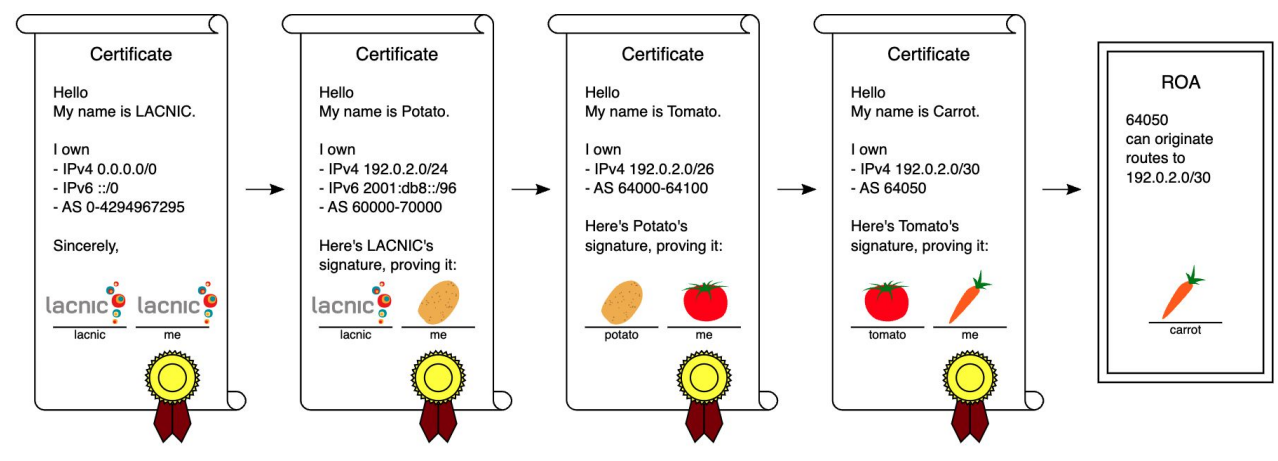
\includegraphics[width=0.85\textwidth]{immagini/NET_09/img.png}
\caption{Processo di creazione e validazione di una ROA: un AS riceve una certificazione firmata da un altro AS per provare l'autorizzazione a originare un prefisso IP. La ROA permette di verificare che un AS possa originare il traffico per determinati prefissi IP.}
\label{fig:rpki-roa-process}
\end{figure}

\subsubsection{Distribuzione dei dati: validator/cache e RTR}
Le ROA non vengono trasportate dentro BGP. Operativamente, i validator scaricano e validano i repository RPKI e producono una vista consistente, poi resa disponibile ai router tramite un meccanismo dedicato (cache server e protocollo RTR). In questo modo i router consumano una lista già validata di tuple \{prefisso, \texttt{maxlength}, origin AS\} e possono fare un controllo locale efficiente durante il processing degli UPDATE.

\begin{figure}[H]
\centering
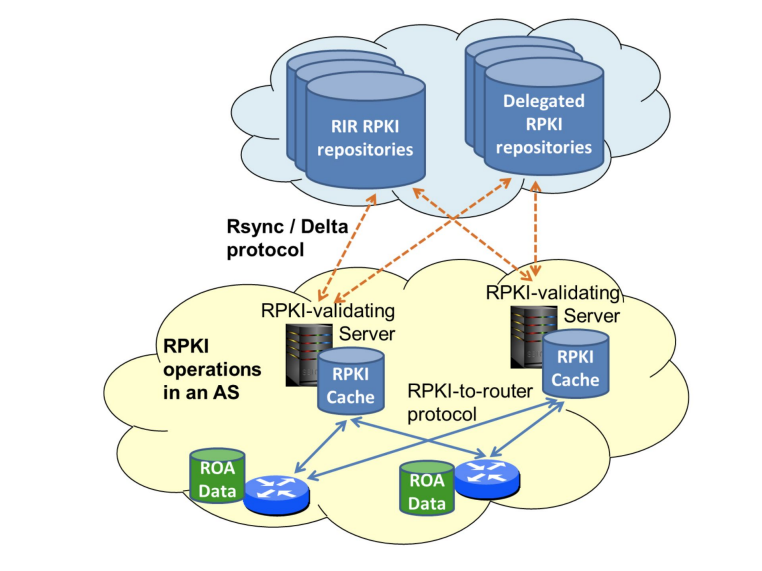
\includegraphics[width=0.88\textwidth]{immagini/NET_09/fig_rpki_retrieval_cache_rtr.png}
\caption{Flusso operativo RPKI: i validator recuperano e validano gli oggetti dai repository (rsync/RRDP) e pubblicano una vista consistente; i router consumano le VRP tramite protocollo RTR per la \emph{origin validation}.}
\label{fig:rpki-retrieval-cache-rtr}
\end{figure}

\subsubsection{Esiti di validazione e uso nelle policy locali}
Con la BGP Origin Validation, ogni rotta viene classificata come \texttt{Valid}, \texttt{Invalid} o \texttt{NotFound}. Il punto chiave è che l’uso di questi risultati è una scelta locale dell’operatore: si può partire da una modalità di sola marcatura (tag-only), introdurre preferenze per le rotte valide (prefer-valid), fino allo scarto delle rotte invalide (drop-invalid). In deployment parziale è normale osservare molte rotte \texttt{NotFound}: per questo, nella pratica si combina RPKI con altre fonti (IRR e dati contrattuali) per ottenere filtri robusti senza compromettere la reachability.

\begin{figure}[H]
\centering
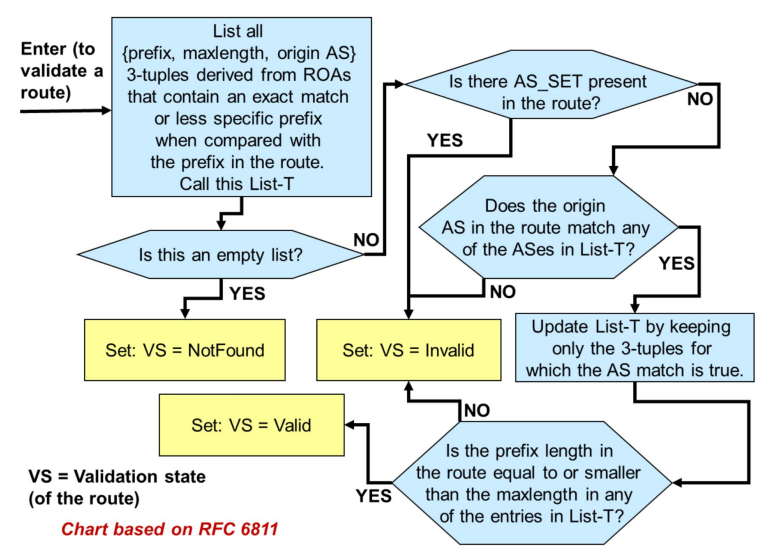
\includegraphics[width=0.90\textwidth]{immagini/NET_09/fig_origin_validation_algorithm.png}
\caption{Schema dell’algoritmo di \emph{BGP Origin Validation}: costruzione dell’insieme di VRP applicabili e classificazione della rotta in \texttt{Valid}, \texttt{Invalid} o \texttt{NotFound}.}
\label{fig:bgp-origin-validation-algorithm}
\end{figure}

\subsection{Limiti dell’origin validation e protezione dell’AS\_PATH}

\subsubsection{Forged-origin hijacks: perché la sola origin validation non basta}
La origin validation verifica il binding \emph{prefisso--origin AS}, ma non garantisce che il cammino dichiarato sia autentico. Un avversario può costruire annunci che risultano ``plausibili'' dal punto di vista dell’origine, inserendo nel path un ASN autorizzato da una ROA per quel prefisso. In questi casi, l’annuncio può risultare \texttt{Valid} pur inducendo traffico verso l’attaccante (che resta il next-hop reale dell’UPDATE). L’efficacia aumenta se l’attaccante combina la forgia dell’origine con un prefisso più specifico ammesso dal \texttt{maxlength}, sfruttando il longest prefix match nel data plane.

\begin{figure}[H]
    \centering
    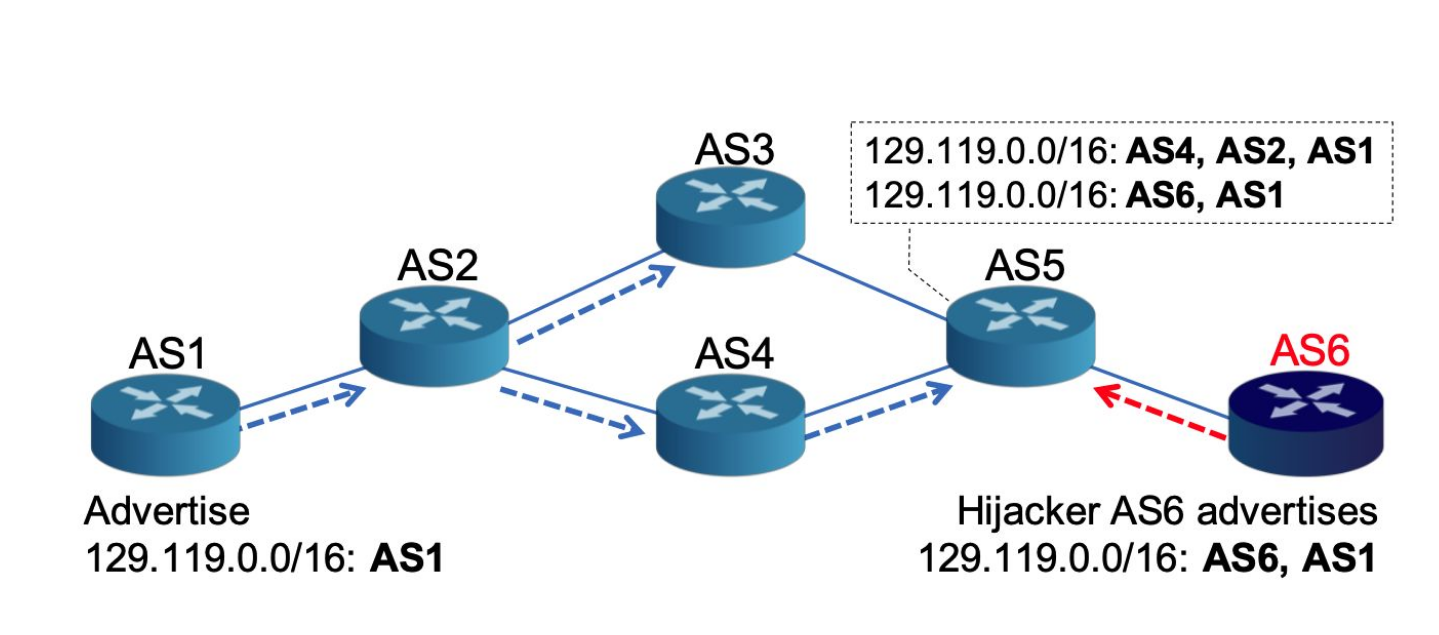
\includegraphics[width=.6\linewidth]{immagini/NET_09/forged}
    \caption{Esempio di \emph{BGP hijacking}: un Autonomous System malevolo annuncia falsamente un prefisso inducendo altri AS a selezionare un percorso non legittimo e dirottando il traffico destinato all’AS originario.}
    \label{fig:forged}
\end{figure}

\subsubsection{BGPsec / Path Validation: idea generale}
Per coprire il limite sull’\texttt{AS\_PATH}, BGPsec introduce firme lungo il cammino: ogni AS firma l’UPDATE che propaga, vincolando le informazioni rilevanti e la sequenza di AS attraversati. In questo modo, rimozioni o inserimenti non autorizzati di hop (ad esempio per accorciare fraudolentemente il path) diventano rilevabili perché romperebbero la verifica delle firme.

\begin{figure}[H]
\centering
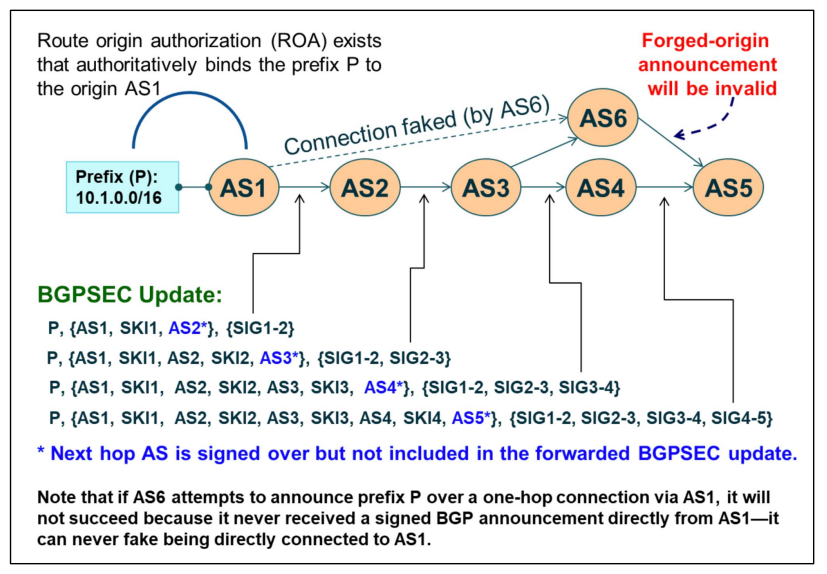
\includegraphics[width=0.80\textwidth]{immagini/NET_09/0ace4c3a-d55e-4b21-b6e2-7dc380925c2f.png}
\caption{Diagramma di flusso per la validazione del path in BGPsec: ogni AS firma i messaggi BGP lungo il cammino, garantendo l'integrità e l'autenticità del percorso.}
\label{fig:bgpsec-path-validation}
\end{figure}

\subsection{Mitigazione dei route leaks: best practice e approcci ``crypto''}

\subsubsection{Prevenzione intra-AS: tagging ingress-to-egress con BGP large communities}
Una best practice molto diffusa per ridurre i route leaks all’interno del proprio AS è marcare gli UPDATE in ingresso con un tag (tipicamente una \emph{BGP large community}) che indica da quale tipo di relazione la rotta è stata appresa (customer, peer laterale, transit provider, originata localmente). Il tag viene poi usato in uscita per applicare export policy robuste e semplici: rotte apprese da customer possono essere esportate più liberamente, mentre rotte apprese da peer o provider devono essere esportate solo verso customer. L’idea è rendere difficile una propagazione “oltre scope” anche in presenza di configurazioni complesse.

\subsubsection{Mitigazione inter-AS: detection e contenimento}
Quando un leak esce comunque dall’AS che lo origina, l’obiettivo diventa identificarlo e contenerlo dopo l’inizio della propagazione. In questo modello, il peer AS (o AS successivi lungo il path) dovrebbe poter riconoscere che un annuncio è incoerente con le relazioni attese e trattarlo in modo conservativo, impedendo ulteriore propagazione e riducendo l’impatto globale.

\subsubsection{ASPA: certificare relazioni provider/customer e (parziale) validazione del path}
ASPA estende l’uso di RPKI oltre la validazione dell’origine, certificando relazioni provider/customer. Per ogni AS si pubblica un oggetto firmato che elenca i provider autorizzati; l’informazione può essere usata per verificare se un AS\_PATH è coerente con relazioni attese e, quindi, per individuare pattern tipici di route leak.

\subsubsection{Limiti di ASPA e complementarità con BGPsec}
ASPA impone vincoli sulle relazioni tra AS adiacenti nel path, ma non fornisce integrità completa dell’\texttt{AS\_PATH}. In alcuni casi selezionati, un avversario può modificare il path (ad esempio accorciandolo) in modo da mantenere una sequenza ancora coerente con le relazioni attestabili, rendendo l’anomalia più difficile da rilevare. Per questo, ASPA è da considerare complementare a BGPsec: ASPA migliora la detection dei leak in modo pragmatico, mentre BGPsec rafforza l’integrità crittografica del cammino.

\newpage
{\LARGE \textbf{Laboratorio}} \\[0.5em]
\subsection{Laboratorio: BGP Security con Kathara, FRR e RPKI (sub-prefix hijack + mitigazione)}

\paragraph{Obiettivo.}
Il laboratorio mostra un attacco di \textbf{sub-prefix hijacking} in una topologia emulata e verifica la mitigazione tramite \textbf{RPKI + BGP Origin Validation}. L’idea è osservare che, senza validazione, il più-specifico dell’attaccante viene preferito per longest prefix match, mentre con una policy \emph{drop-invalid} l’annuncio malevolo non viene installato né propagato.

\paragraph{Strumenti.}
Kathara per l’emulazione, FRRouting per la configurazione BGP, Krill per pubblicare ROA e un validator/cache (es.\ Routinator) per fornire ai router i dati validati tramite RTR.

\begin{figure}[H]
\centering
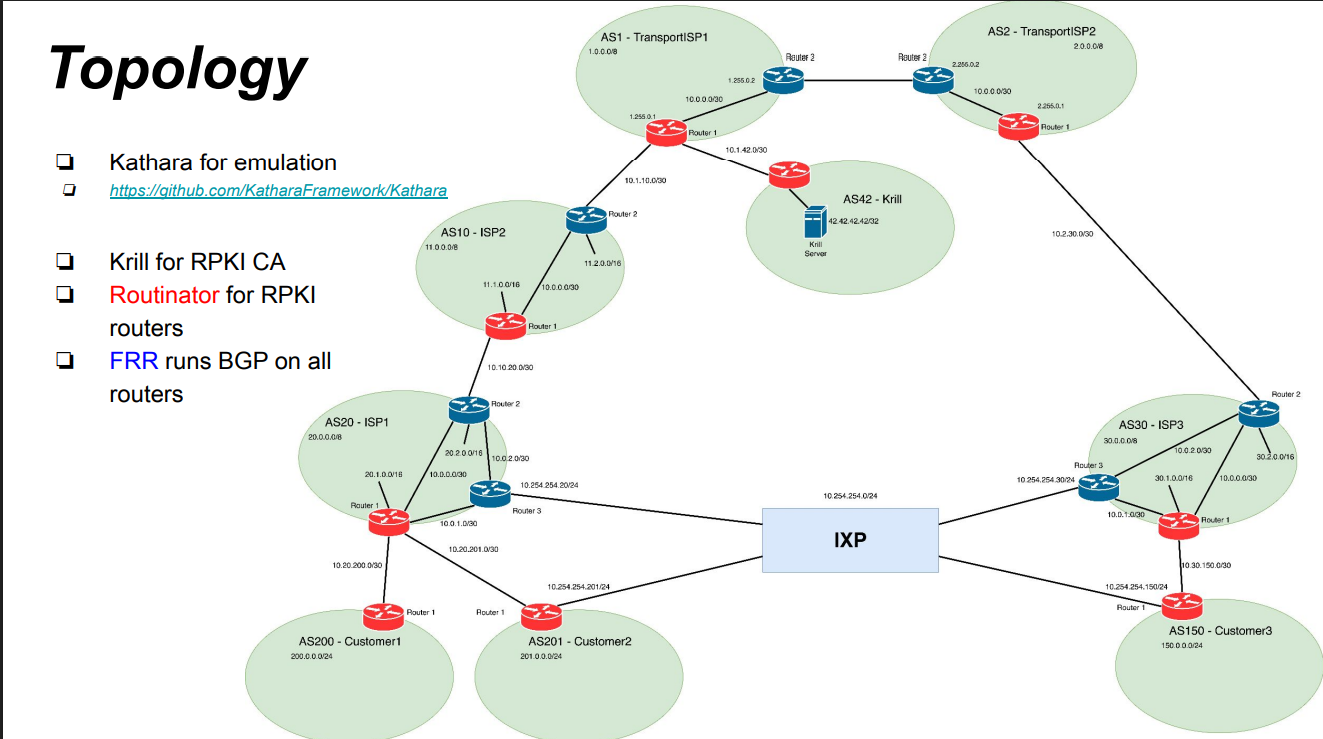
\includegraphics[width=0.55\textwidth]{immagini/NET_09/lab_rpki_hijack_topology.png}
\caption{Scenario di laboratorio: prefisso legittimo, attaccante e sorgente del traffico con transito intermedio.}
\end{figure}

\paragraph{Sequenza sperimentale.}
Si esegue prima lo scenario \textbf{senza RPKI}: si verifica il path legittimo da Customer 1 verso la rete di Customer 3, poi Customer 2 annuncia un prefisso più specifico e si osserva che il path cambia e il traffico viene attratto verso l’attaccante. Successivamente si abilita \textbf{RPKI}: si pubblica una ROA per il prefisso legittimo con \texttt{maxlength} impostato in modo da rendere \textbf{Invalid} il più-specifico dell’attaccante, si collega FRR al validator RTR e si applica una policy \emph{drop-invalid}. Ripetendo l’attacco, l’annuncio malevolo non risulta più efficace e il percorso verso la destinazione torna coerente con l’owner legittimo.
